\chapter{System calibration} 
 
         
For performing non-metric reconstruction only point-to-point correspondences between camera and projector are needed to perform triangulation[3]. But to relate the depth computed using triangulation with physical metrics such as 'mm', 'cm' etc there is need to relate the camera and projector geometry with physical measurement units, this task is accomplished by process of System calibration.  Calibration is a process of determining intrinsic and extrinsic characteristics of the imaging devices(camera and projector in our case). Intrinsic characteristics include focal length, coordinates of principal points of lens used in camera and projectors, image axis skew coefficients and lens distortion coefficients. Extrinsic characteristics include rigid-body transformations that can transform a point represented in World-coordinate system to individual coordinates systems of camera and projector. \newline 

 
Above discussion clearly implies the need to establish defining equations which relate a real-world three dimensional point(with coordinates expressed in \textit{physical} units) with pixel coordinates in camera(or projector). For this purpose a projective model of camera which applies to projector as well is introduced in the next section which clearly describes the problem of calibration, following which the current approaches and the approach used in this work to solve this problem will be reviewed. In the end, a note on \textit{relative extrinsic calibration} of projector-camera system is mentioned, which is a process of determining relative rotation and translation of camera and projector coordinate systems which in simple words means to determine the relative orientation and position of camera with respect to projector or vice-versa.   
  
\section{Camera model}   
Camera model is a concise mathematical abstraction of the internal(i.e., its optics and sensor arrangement) and external(i.e., its position relative to a scene) geometry of camera which is responsible for the imaging process. In this section, these geometric parameters will be described and hence the imaging process. Camera model described here is referred from seminal paper by [8]. Other calibration techniques also follow variants of this formulation. Relatively recent work in [9] has shown projector to be \textit{inverse-camera} hence further discussion on camera calibration holds equally to projector as well. Section 2.4.2 will describe how  projector was calibrated similar to camera with a real example. In next subsection the coordinate-systems which are relevant for geometric modeling of imaging process under consideration will be described.  
  
\subsection{Graphical abstraction}  
In this subsection the graphical model of camera depicting coordinate systems involved in transforming a real world 3D point to camera 2D coordinate representation will be described.
   
\paragraph{World-coordinate system.}  
World-coordinate system defines the reference frame in the real world that will be used for defining the positions of object in scene in physical units. Typically any location in the real scene can be used as origin for world coordinate system axes. For example in this work world coordinate system origin was assumed to be present at a corner on a wall.  
  
\paragraph{Camera-coordinate system.}  
This is a 3D reference coordinate-system internal to camera, it is similar to world coordinate system since it also works in physical units. Its origin is assumed to be at center of projection of camera. It is used to generate 3D interpretation of the scene from camera viewpoint.  
  
\paragraph{Image-coordinate system.}  
This is a 2D reference coordinate-system for indexing points in the real-image. Note here \textit{real} means that it can take real values as coordinates. It is used to index the points in perspective projection of 3D world.  
  
\paragraph{Computer-frame coordinate system.}  
This is a 2D reference coordinate-system which indexes pixels in the computer-frame. It can only have integral coordinates. Images with which we normally interact are indexed with respect to this coordinate system. \newline  
  
Figure~\ref{fig:coordinate_systems}\footnote{Figure source: Refer~\cite{8}} illustrates the coordinate systems except computer-frame coordinate system since it is not geometrically connected with other coordinate systems:  
  
%\begin{figure}[hb]  
%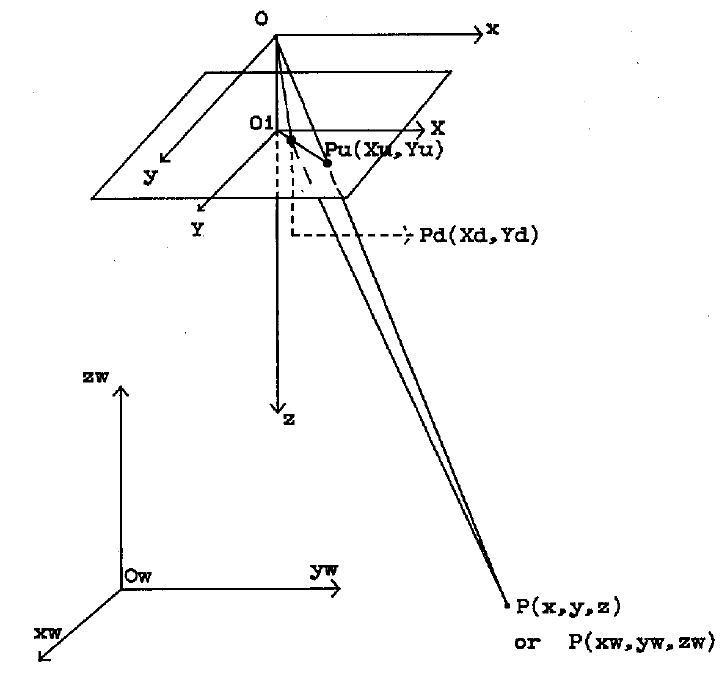
\includegraphics[width=10cm,height=10cm]{../img_source/coordinate_systems.jpg}  
%\caption{Transformation of a real world 3D point from world coordinate system to computer-buffer coordinate system}  
%\label{fig:coordinate_systems}
%\end{figure}  

\begin{figure}[ht]
\centering
\begin{tikzpicture}
% world coordinate system
\draw[->] (0,0)--(0,3);%Y
\draw[->] (0,0)--(3,0);%X
\draw[->] (0,0)--(-1.5,-1.5);%Z
\node[below] at (0,0) {\textbf{$O_w$}};
\node[below] at (3,0) {\textbf{$X_w$}};
\node[left] at (0,3) {\textbf{$Y_w$}};
\node[below] at (-1.0,-1.5) {\textbf{$Z_w$}};

% camera coordinate system
\draw[->] (2,9)--(2,4);%Z
\draw[->] (2,9)--(5,9);%X
\draw[->] (2,9)--(1,6);%Y
\node[left] at (2,9) {\textbf{$O_c$}};
\node[above] at (5,9) {\textbf{$X_c$}};
\node[below] at (2,4) {\textbf{$Z_c$}};
\node[below] at (1,6) {\textbf{$Y_c$}};

% camera-image coordinate system
\draw (0.5,8)--(6,8);
\draw (0.5,8)--(-0.5,6);
\draw (6,8)--(5,6);
\draw (-0.5,6)--(5,6);

\node[left] at (2,7.5) {\textbf{$O_i$}};
\fill [black] (2,7.5) circle[radius=2pt];

\draw[->] (2,7.5)--(4,7.5);
\draw[->] (2,7.5)--(1,4.5);
\node[below] at (4,7.5){\textbf{$X_i$}};
\node[left] at (1,4.5){\textbf{$Y_i$}};

%3d point
\node[below] at (7,-1){\textbf{$P$}};
\fill [black] (7,-1) circle[radius=2pt];

\draw (7,-1)--(2.9,7.3);
\fill[black] (2.9,7.3) circle[radius=2pt];
\node[below] at (2.9,7.3) {\textbf{$P_u$}};

\draw (2.9,7.3)--(2,9);


\node[below] at (2.5,6.9) {\textbf{$P_d$}};
\fill[black] (2.5,6.9) circle[radius=2pt];

\draw (7,-1)--(2.5,6.9);
\draw (2.5,6.9)--(2,9);

\end{tikzpicture}
\caption{Transformation of a real world 3D point from world coordinate system to computer-buffer coordinate system}  
\label{fig:coordinate_systems}
\end{figure}  


Here points $O_w,O_c$ and $O_i$ represent origins of world,camera and real-image coordinate systems respectively. Further, axes $X_w,Y_w$ and $Z_w$ represent the world-coordinate system, axes $X_c,Y_c$ and $Z_c$ denote the camera coordinate system, similarly axes $X_i$ and $Y_i$ show the 2D real-image coordinate system, $P$ is a real-world point, $P_u$ is the ideal projection of $P$ on real-image plane(i.e., image-coordinate system), $P_d$ is corresponding distorted projection which differ from $P_u$ due to practical imperfections in camera system. Equations relating these coordinate systems are described in the following paragraphs of this section.  
  
\subsection{Mathematical abstraction}  
In this subsection, the actual mathematical form of camera imaging process which is used for transforming a real-world 3D point to a computer-buffer pixel will be sequentially described. This involves a series of coordinate transformations which are described here.   

\paragraph{1.Rigid body transformations from object world-coordinate system to camera coordinate system.}  
Points in the world-coordinate coordinates system (x\textsubscript{w},y\textsubscript{w},z\textsubscript{w}) are transformed to the camera-coordinate system (x\textsubscript{c},y\textsubscript{c},z\textsubscript{c}). To model this process, rotation(R) and translation(T) matrices are used as:  
  
\begin{equation}  
\begin{bmatrix}  
x_c \\  
y_c \\  
z_c  
\end{bmatrix}  
=  
R*   \begin{bmatrix}  
      x_w \\  
      y_w \\  
      z_w  
      \end{bmatrix}  
+T  
\end{equation}  
where $R=\begin{bmatrix}  
         r_{1,1} & r_{1,2} & r_{1,3} \\  
         r_{2,1} & r_{2,2} & r_{2,3} \\  
         r_{3,1} & r_{3,2} & r_{3,3}   
         \end{bmatrix}$  
,$T=\begin{bmatrix}  
    t_x \\  
    t_y \\  
    t_z  
   \end{bmatrix}$ \newline  
  
  
Rotation and translation parameters are called \textit{extrinsic parameters} of camera/projector. It should be noted here that rotation followed by translation is used since it ensures unique transformations, whereas translation followed by rotation can result in multiple possible transformations[8].  
  
  
  
\paragraph{2.Perspective transformation from camera-coordinates to real-image coordinates.}  
In this step, 3D scene as viewed from camera-coordinate origin is perspective projected to a plane. Hence it is a 3D to 2D transformation resulting in loss of Z-coordinate(i.e., depth) since multiple points are projected onto same point in the image-plane. Following equations describe this process:  
  
\begin{equation}  
\begin{bmatrix}  
x_u \\  
y_u  
\end{bmatrix}  
=\bigg(\frac{f}{z_c}\bigg)*  
\begin{bmatrix}  
x_c \\  
y_c  
\end{bmatrix}  
\end{equation}  
  
\noindent  
where \textit{f} represents the focal length of camera/projector lens. (x\textsubscript{u},y\textsubscript{u}) is the perspective projection of point (x\textsubscript{c},y\textsubscript{c},z\textsubscript{c}) on real-image plane.  
  
\paragraph{3.Radial and tangential lens distortion.}  
In this step, real-image coordinates are distorted due to radially imperfections in practical lens which is characterized by \textit{radial distortion} and oblique alignment of principal plane of lens and sensor-plane which is characterized by \textit{tangential distortion}. Although Tsai's work only accounted for radial distortions subsequent works have accounted for tangential[10] and prism distortions[11] also in an attempt to increase the accuracy of estimated calibration parameters further. Following equations describes the effect of radial and tangential distortion on \textit{ideal} image coordinates:  
\begin{equation}  
\begin{aligned}
& x_d=x_u(1+k_1r^2+k_2r^4+k_3r^6+...)+2p_1x_uy_u+p_2(r^2+2x_u) \\
& y_d=y_u(1+k_1r^2+k_2r^4+k_3r^6+...)+2p_2x_uy_u+p_1(r^2+2y_u)
\end{aligned}
\end{equation}  
\noindent  
where,\newline
$(x_d,y_d)$: distorted image coordinates\newline
$(k_1,k_2,k_3)$: radial distortion coefficients\newline
$(p_1,p_2)$: tangential distortion coefficients\newline
$r=\sqrt[2]{X_u^2+Y_u^2}$
  
\paragraph{4.Transforming real-image coordinates to computer-frame coordinates.}  
Finally to map 3D world-coordinates to frame coordinates of camera, i.e., the pixels that we see, following equations are assumed:  
\begin{equation}  
\begin{bmatrix}  
x_f \\  
y_f  
\end{bmatrix}  
=\begin{bmatrix}  
s_x*(d_x^{'})^{-1}*x_d\\  
d_y^{-1}*y_d  
\end{bmatrix}   
+\begin{bmatrix}  
C_x \\  
C_y  
\end{bmatrix}  
\end{equation}  
\noindent  
where,\newline  
$(x_f,y_f)$:computer frame-buffer coordinates for point $(x_d,y_d)$ \newline  
$s_x$:uncertainty image-scale factor \newline  
$d_x$:center-to-center distance between sensor cells along X-direction\newline  
$N_{cx}$:Number of sensors along X-direction\newline  
$N_{fx}$:Number of pixels along X-line sampled by computer\newline  
$d_x^{'}=d_x*\left(\frac{N_{cx}}{N_{fx}}\right)$\newline\newline  
It should be noted that at full camera resolution there is one-to-one relation between number of sensor elements and number of pixels in computer-frame buffer hence $N_{cx}=N_{fx}$ and hence $d_x^{'}=d_x$ but in general $d_x^{'}>=d_x$. [8] attributed $s_x$ to be due to  possibility of mismatch between camera image acquisition hardware and camera scanning hardware. Figure~\ref{fig:cam_model_pipeline}\footnote{Figure source: Refer~\cite{8}} illustrates the complete imaging process. 
%\begin{figure}[ht]  
%\centering  
%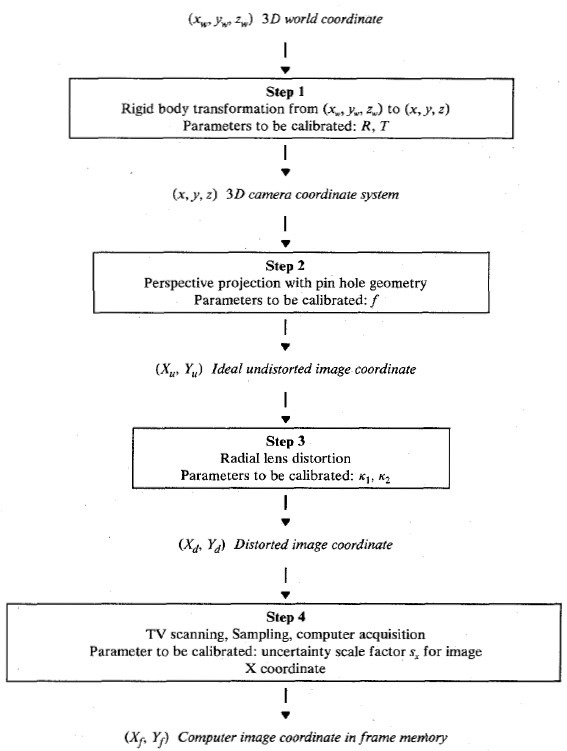
\includegraphics[width=10cm,height=14cm]{../img_source/cam_model_pipeline.jpg}  
%\caption{Camera model pipeline}  
%\label{fig:cam_model_pipeline}
%\end{figure}  
\begin{figure}
\centering
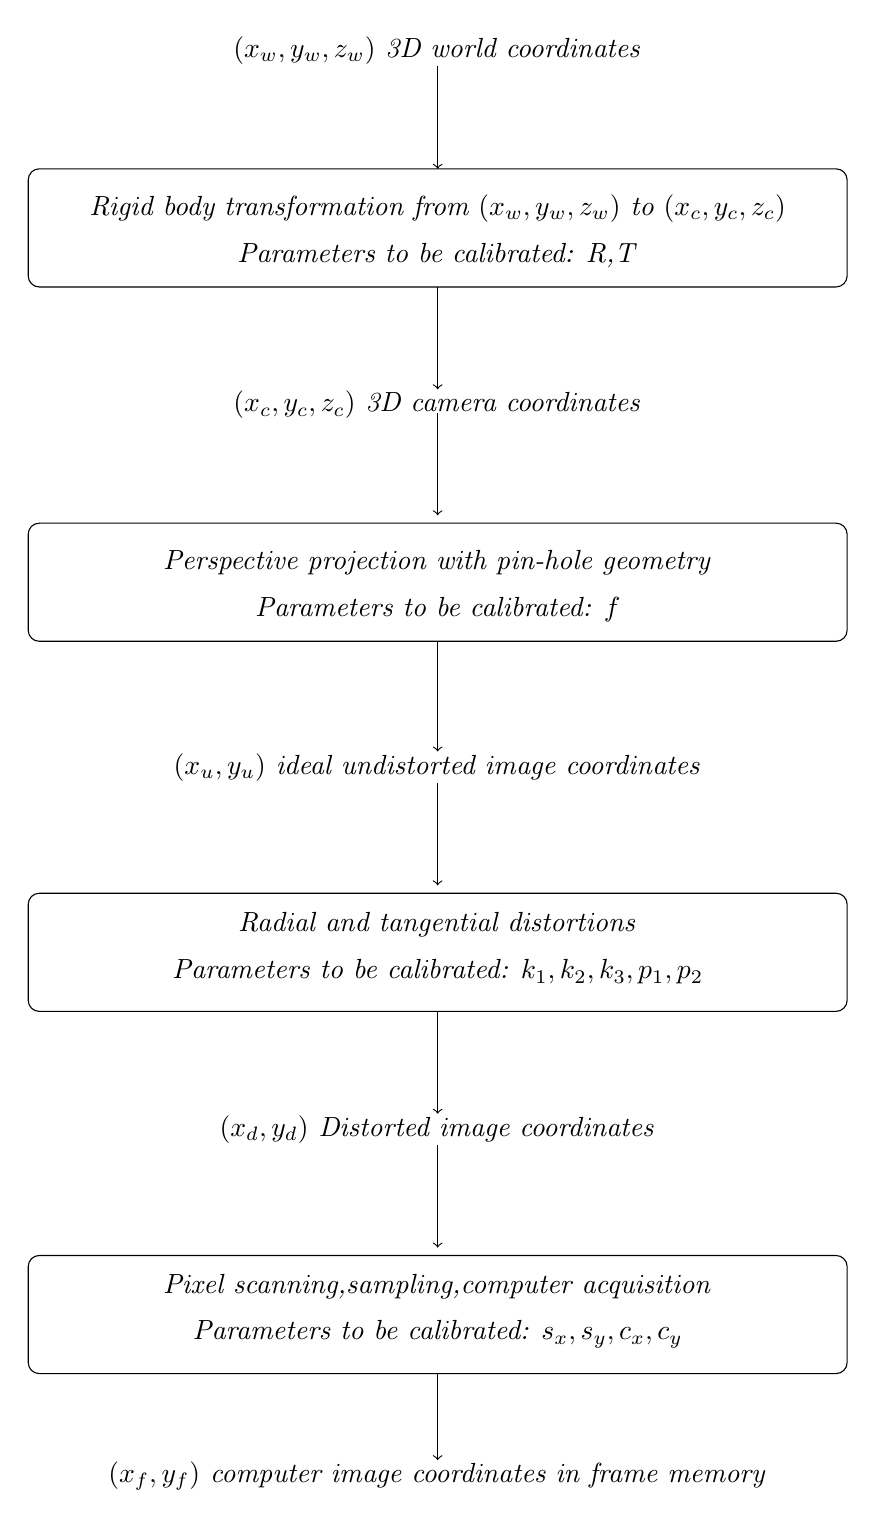
\begin{tikzpicture}
\node at (0,0) {\textit{$(x_w,y_w,z_w)$ 3D world coordinates}};
\draw[->] (0,-0.2)--(0,-1.5);
\draw[rounded corners] (-5.2,-1.5) rectangle (5.2,-3);
\node at (0,-2.0){\textit{Rigid body transformation from $(x_w,y_w,z_w)$ to $(x_c,y_c,z_c)$}};
\node at (0,-2.6) {\textit{Parameters to be calibrated: R,T}};

\draw[->] (0,-3)--(0,-4.3);
\node at (0,-4.5) {\textit{$(x_c,y_c,z_c)$ 3D camera coordinates}};
\draw[->] (0,-4.6)--(0,-5.9);
\draw[rounded corners] (-5.2,-6.0) rectangle (5.2,-7.5);
\node at (0,-6.5) {\textit{Perspective projection with pin-hole geometry}}; \node at (0,-7.1) {\textit{Parameters to be calibrated: $f$}};

\draw[->] (0,-7.5)--(0,-8.9);
\node at (0,-9.1) {\textit{$(x_u,y_u)$ ideal undistorted image coordinates}};

\draw[->] (0,-9.3)--(0,-10.6);
\draw[rounded corners] (-5.2,-10.7) rectangle (5.2,-12.2);
\node at (0,-11.1) {\textit{Radial and tangential distortions}};
\node at (0,-11.7) {\textit{Parameters to be calibrated: $k_1,k_2,k_3,p_1,p_2$}};

\draw[->] (0,-12.2)--(0,-13.5);
\node at (0,-13.7) {\textit{$(x_d,y_d)$ Distorted image coordinates}};
\draw[->] (0,-13.9)--(0,-15.2);
\draw[rounded corners] (-5.2,-15.3) rectangle (5.2,-16.8);

\node at (0,-15.7) {\textit{Pixel scanning,sampling,computer acquisition}}; 
\node at (0,-16.3) {\textit{Parameters to be calibrated: $s_x,s_y,c_x,c_y$}};

\draw[->] (0,-16.8)--(0,-17.9);
\node at (0,-18.1) {\textit{$(x_f,y_f)$ computer image coordinates in frame memory}};
\end{tikzpicture}
\caption{Camera model pipeline}  
\label{fig:cam_model_pipeline}
\end{figure}

\noindent  
So based on above discussion we can deduce that to define the geometric imaging process of camera(or projector) we have to estimate following parameters:
\begin{enumerate}  
\item Internal parameters:
\begin{enumerate}
\item Camera lens focal length
\item Position of principal point on the real-image plane
\item Lens distortion parameters
\end{enumerate}
\item External parameters:
\begin{enumerate}
\item Rotation between camera-coordinate system and world-coordinate system  
\item Translation between camera-coordinate system and world-coordinate system  
\end{enumerate}
\end{enumerate}  
  
  
  
\section{Current approaches:A review}  
A taxonomy was proposed by [10] for camera calibration approaches based on their requirement of additional calibration objects as:  
\paragraph{a) Photogrammetric calibration.}  
These techniques perform camera calibration by observing a calibration object. Calibration object can be any object with known geometry i.e., we know world-coordinates of feature-points on the object that we want to use for calibration. In this category many techniques for both 3D and 2D calibration objects were proposed. For example use of 3D calibration object with three orthogonal planes or planar calibration rigs with known translation across its views have been used for calibration[8] although requiring elaborate setup for calibration and often time-consuming.  
\paragraph{b) Self-calibration.}  
These techniques are more flexible than photogrammetric techniques in that they do not require an explicit calibration rig for calibration, but by moving the camera across a static rigid scene they determine constraints on internal parameters of camera that can be used for calibration[12][13]. Other than these techniques there are techniques that do not fall into these categories
such as camera calibration using vanishing points for orthogonal directions[14], calibration from pure rotation[15]. In this work, a photogrammetric method for camera and projector calibration was used. Following paragraphs will briefly describe the details of some highly cited and practically used algorithms in chronological order.\newline  
  
\paragraph{R.Y.Tsai's algorithm.}  
Tsai's algorithm restricts the lens-distortion effects to only radial distortion and do not account for skewness or lack of orthogonality of projection. Calibration was divided in 2 separate stages. In first stage all extrinsic parameters except for $t_z$ are computed using the \textit{Radial alignment constraint(RAC)} shown in figure~\ref{fig:rac}\footnote{Figure source: Refer~\cite{16}}. If assumed lens distortion is only \textit{radial}, then the direction of vector $O_iP_d$ remains unchanged and is parallel to vector $P_{oz}P_w$. Tsai showed that RAC is independent of magnitude of effective focal length, radial distortion coefficients and position of point $P_w$ along z-axis. He further proved that this constraint is sufficient to estimate 3D rotation and translation of $P_w$ along X and Y axes. \newline   
\begin{figure}[ht]  
\centering  
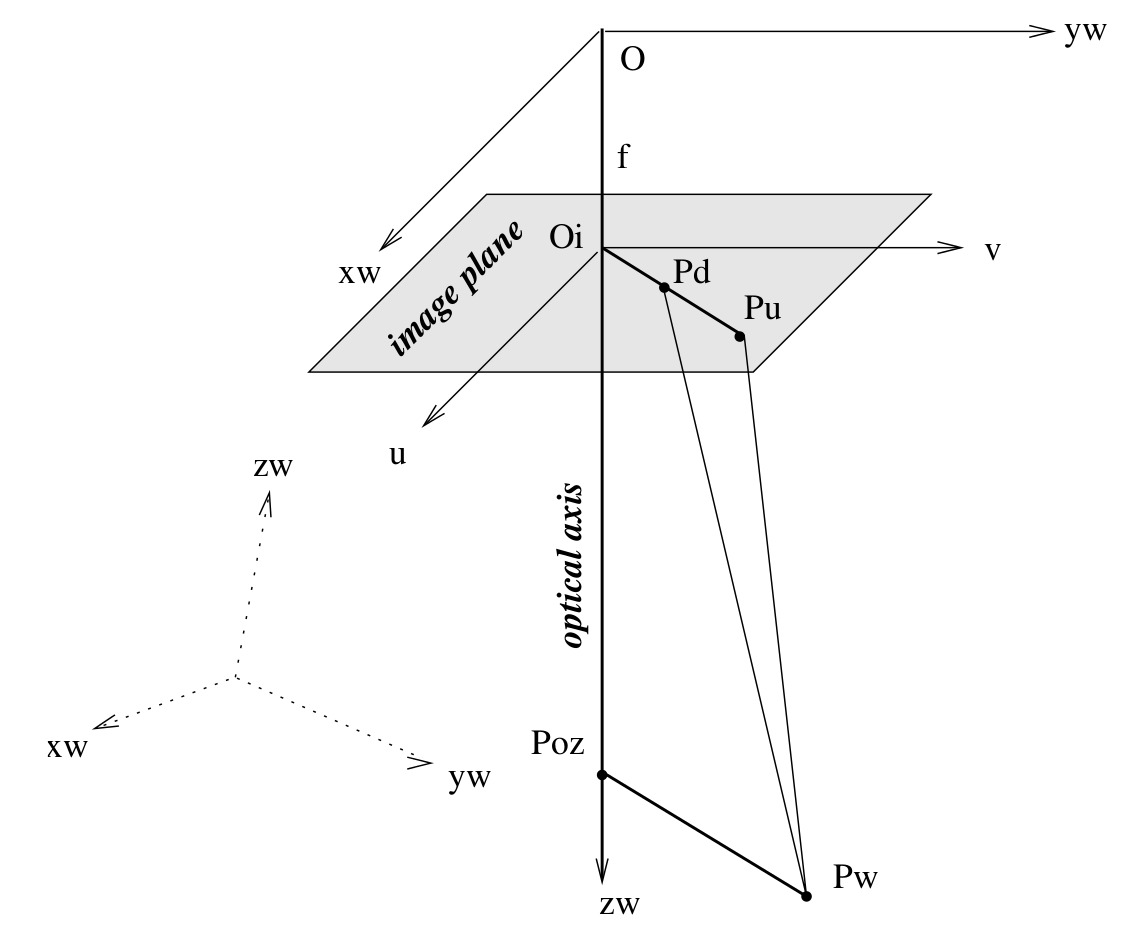
\includegraphics[width=13cm,height=10cm]{../img_source/tsai_rac.jpg}  
\caption{Radial alignment constraint used in Tsai's algorithm}  
\label{fig:rac}
\end{figure}  
  
\noindent  
In second stage effective focal length, distortion coefficients and $t_z$ are estimated using non-linear optimization.  
  
  
\paragraph{Z.Zhang's algorithm.}  
Z.Zhang proposed a plane based camera calibration algorithm[10]. It first acquires real-world coordinate to camera image coordinate correspondences using planar calibration board. Then it estimates all intrinsic and extrinsic parameters using a closed-form solution. This closed form solution assumes zero lens distortion and is based on two constraints on intrinsic parameters derived from the \textit{orthonormality} of rotation vector expressed in equations 2.5,2.6.  
\begin{equation}  
h_1^TA^{-T}A^{-1}h_2=0  
\end{equation}  
\begin{equation}  
h_1^TA^{-T}A^{-1}h_1=h_2^{T}A^{-T}A^{-1}h_2  
\end{equation}  
\noindent  
where,\newline  
$h_i$: $i^{th}$ column vector of Homography\newline  
$A$: Camera projective matrix\newline  
  

Further, the coefficients of radial distortion $k_1,k_2$ are estimated by solving linear least squares expressed in equation 2.7.  
\begin{equation}  
\begin{bmatrix}  
(u-u_0)(x^2+y^2) & (u-u_0)(x^2+y^2)^2 \\  
(v-v_0)(x^2+y^2) & (v-v_0)(x^2+y^2)^2  
\end{bmatrix}  
\begin{bmatrix}  
k_1 \\  
k_2  
\end{bmatrix}  
=\begin{bmatrix}  
u'-u \\  
v'-v  
\end{bmatrix}  
\end{equation}\newline  
\noindent  
where,\newline  
$(u,v)$: ideal pixel image coordinates\newline  
$(u_0,v_0)$: coordinates of principal point\newline  
$(x,y)$: ideal normalized image coordinates\newline  
  

\noindent  
Estimated values of all parameters are considered as initial input for non-linear least squares minimization which minimizes expression in equation 2.8.  
\begin{equation}  
\sum_{i=1}^{m}\sum_{j=1}^{n}||m_{ij}-m'(A,k_1,k_2,R_i,t_i,M_j)||^2  
\end{equation}\newline  
\noindent  
where,\newline  
$m$: Total number of features on the calibration board \newline  
$n$: Total number views of planar calibration board \newline  
$M_j$: 3D coordinates of $j^{th}$ feature point on calibration board\newline  
$m_{ij}$: True 2D coordinates of projection of $M_j$ in camera image\newline   
$m'$: Estimated 2D coordinates for $M_j$ using calibration parameters\newline  
$R_i$: Rotation parameters for $i^{th}$ view used for calibration\newline  
$t_i$: Translation parameters for $i^{th}$ view used for calibration\newline  
  
\paragraph{J.Heikkila et al.'s algorithm.}  
This algorithm assumes a more elaborate camera model which includes both radial and tangential components as lens distortion coefficients. It first linearizes the camera model by ignoring lens distortion coefficients and performs linear parameter estimation using Direct Linear Transformation(DLT)[17]. Equation 2-9 shows the linear model solved using DLT method.\newline  
\begin{equation}  
La=0  
\end{equation}\newline  
\noindent  
where,\newline   
a=$\begin{bmatrix}  
a_{1,1} & a_{1,2} & a_{1,3} & a_{1,4} & a_{2,1} & a_{2,2} & a_{2,3} & a_{2,4} & a_{3,1} & a_{3,2} & a_{3,3} & a_{3,4}   
\end{bmatrix}$\newline  
\newline  
L=$\begin{bmatrix}  
X_1 & Y_1 & Z_1 & 1 & 0 & 0 & 0 & 0 & -X_1u_1 & -Y_1u_1 & -Z_1u_1 & -u_1 \\  
0 & 0 & 0 & 0 & X_1 & Y_1 & Z_1 & 1 & -X_1v_1 & -Y_1v_1 & -Z_1v_1 & -v_1 \\    
: & : & : & : &  :  &  :  &  :  & : &   :     &    :    &    :    &   : \\  
X_i & Y_i & Z_i & 1 & 0 & 0 & 0 & 0 & -X_iu_i & -Y_iu_i & -Z_iu_i & -u_i \\  
0 & 0 & 0 & 0 & X_i & Y_i & Z_i & 1 & -X_iv_i & -Y_iv_i & -Z_iv_i & -v_i \\  
: & : & : & : &  :  &  :  &  :  & : &   :     &    :    &    :    &   : \\  
X_n & Y_n & Z_n & 1 & 0 & 0 & 0 & 0 & -X_nu_n & -Y_nu_n & -Z_nu_n & -u_n \\  
0 & 0 & 0 & 0 & X_n & Y_n & Z_n & 1 & -X_nv_n & -Y_nv_n & -Z_nv_n & -v_n   
\end{bmatrix}$ \newline  
\newline  
\newline  
\noindent  
Here, $(X_i,Y_i,Z_i)$ denotes 3D coordinates of $i^{th}$ feature point used in calibration, $(u_i,v_i)$ denotes the corresponding 2D image coordinates, \textit{a} denotes the projective matrix mapping $(X_i,Y_i,Z_i)$ to $(u_i,v_i)$.  
In second step, Gaussian noise model is assumed and a non-linear least square minimization is performed to minimize equation 2-10.\newline    
\begin{equation}  
F=\sum_{i=1}^N\big[(U_i-u_i)^2+(V_i-v_i)^2\big]  
\end{equation}  
\noindent  
where, \textit{N} is the number of observations, $(U_i,V_i)$ are the observed 2D coordinates of $i^{th}$ feature point, $(u_i,v_i)$ are corresponding 2D coordinates estimated using calibration parameters.  
  
  
  
\section{Approach followed in this work}  
For camera and projector calibration an extension of [10] method was used which was first described and developed in [18] and later ported to OpenCV. Unfortunately, author in [18] has not published the details of algorithm except describing the approach to be based on camera model described in [17] and implementation as a variant of [10] hence  
OpenCV documentation other than reading the source code itself is the only source of  
theoretical information on this technique. During this project work, an effort is initiated  
to fully understand the calibration algorithms and effect of each calibration  
parameters on accuracy of 3D reconstruction by actually implementing an algorithm  
so that every input to the algorithm can be changed and its effect seen. For which technique described in [17] was selected and partially implemented. Here a brief outline of camera/projector calibration algorithm implemented in OpenCV/Matlab[18][19] is presented:  
\begin{enumerate}
\item A planar calibration board is selected with known world-coordinates of reference points on it.  
\item Calibration board is shown for multiple views(at least 2) in front of camera by varying its rotation and translation(amount need not be known) with respect to camera and for every pose feature-points are  
detected in camera.  
\item After all such views are captured and feature-points detected, homography for each view is calculated.  
\item Closed form solution of intrinsic parameters from homographies using orthogonality of vanishing points is computed but unlike [10] no initial estimates of distortion coefficients are computed.  
\item Initial estimates of calibration parameters computed earlier are given as input to Maximum likelihood estimator Levenberg-Marquardt algorithm[20] to refine the parameters.Output of this process is a set of calibration parameters which optimally satisfy the maximum likelihood criteria.  
\end{enumerate}

 
\paragraph{Algorithm for extrinsic calibration of camera and projector.}  
Extrinsic parameters relate camera-coordinate system and projector-coordinate system to world-coordinate system. For  
extrinsic calibration, OpenCV[21] performs minimization of re-projection error between  
observed point projections given as input(i.e., image points) and projection computed  
by applying the estimated model to the given object points. Extrinsic parameters that  
minimize this criteria are considered as the optimal pose(Rotation and translation)  
parameters.  
  
\paragraph{A note on Relative calibration of projector and camera.}  
After camera and projector are calibrated extrinsically, there is need to relate their  
coordinate-systems with each other so that a point in projector coordinate-system can  
also be expressed in terms of camera-coordinate system. This is required because of  
an implicit assumption in triangulation is that it requires intersection of optical rays from  
camera and projector, which is possible only if we can express both rays in a common  
coordinate-system either in that of camera or projector. This is achieved  
using our world-coordinate system as a common link between projector and camera.  
Following equations relate camera-coordinate system to projector-coordinate system  
via world-coordinate system[22]:  
\begin{equation}  
\begin{bmatrix}  
P_c \\  
P_p  
\end{bmatrix}  
=\begin{bmatrix}  
R_{wc}*P_w \\  
R_{wp}*P_w  
\end{bmatrix}  
+\begin{bmatrix}  
T_{wc} \\  
T_{wp}  
\end{bmatrix}  
\end{equation}  
hence,\newline  
$P_c=\underbrace{(R_c*R_p^{-1})}_{R_{pc}}*P_p+\underbrace{(T_c-R_c*R_p^{-1}*P_p)}_{T_{pc}}$  
  
\noindent  
where,\newline  
$P_w$:A point in world coordinate system\newline  
$P_c$:Representation of $P_w$ with respect to camera coordinate system\newline  
$P_p$:Representation of $P_w$ with respect to projector coordinate system\newline  
$R_{wc}$:Rotation transformation from world-to-camera coordinate system\newline  
$R_{wp}$:Rotation transformation from world-to-projector coordinate system\newline  
$T_{wc}$:Translation transformation from world-to-camera coordinate system\newline  
$T_{wp}$:Translation transformation from world-to-projector coordinate system\newline  
$R_{pc}$:Rotation transformation from projector-to-camera coordinate system\newline  
$T_{pc}$:Translation transformation from projector-to-camera coordinate system\newline  
  
Here $R_{pc}$ and $T_{pc}$ are the final outcomes which allows us to map a point in projector coordinate system to camera coordinate system which is an requirement for performing stereo-triangulation.  
  
\section{Working of developed system calibration module}  
System calibration is composed of camera calibration, projector calibration and relative extrinsic calibration of camera with respect to projector. A module for system calibration was developed which performs above mentioned functions using OpenCV camera calibration and extrinsic calibration algorithms. This section first describes the system setup and then explains the practical procedure for camera, projector and extrinsic calibration of projector with respect to camera.  
  
\paragraph{System setup.}  
In this work,Logitech Quickcam sphere AF web-cam at 1600X1200 pixels  
resolution was as a capture device, Sharp PG-F200X projector at 1024X768 pixels resolution was used for pattern projection, and 4 markers(shown in figure~\ref{fig:calib_setup} as `black' points) as world coordinate references forming a  
rectangular region of 1900mm X 1700mm and a physical checkerboard with square  
size 25.6mm arranged in a 10X8 square grid. Figure~\ref{fig:calib_setup} shows setup of our 3D  
scanner system:\newline  
  
\begin{figure}[htbp]  
\centering  
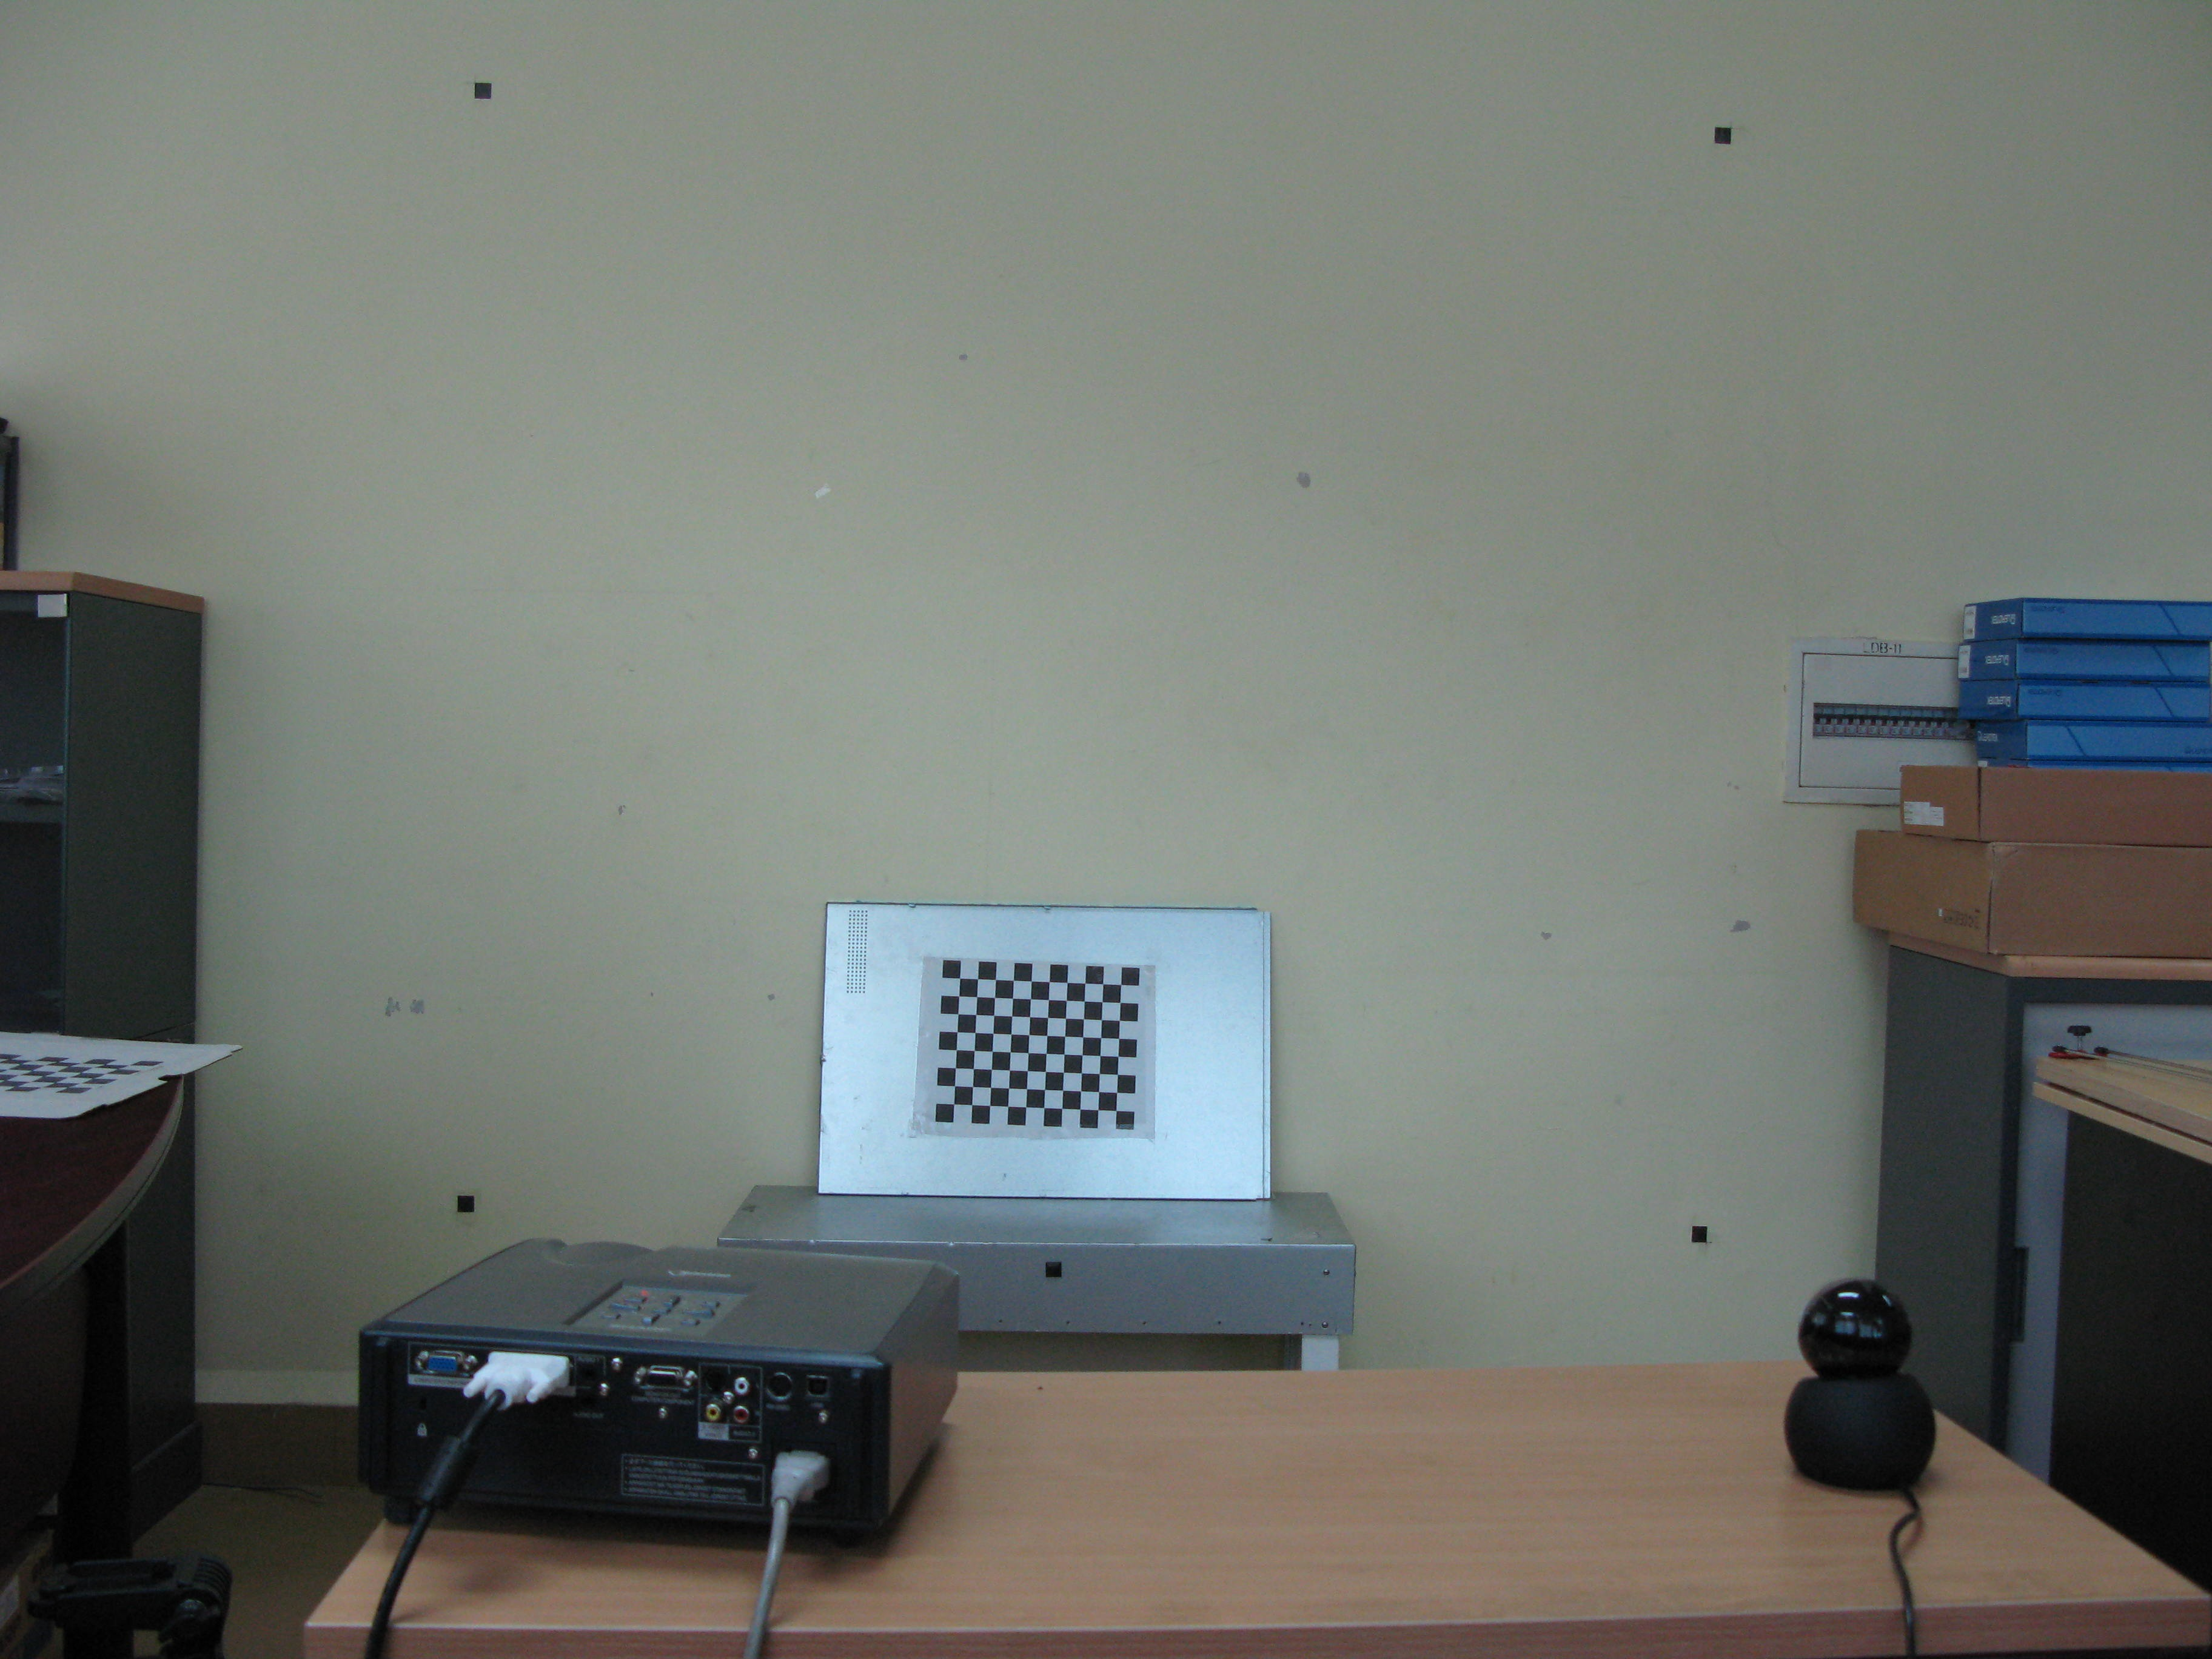
\includegraphics[width=10cm,height=8cm]{../img_source/system_setup.jpg}  
\caption{System setup}
\label{fig:calib_setup}  
\end{figure}  
  
\subsection{Camera calibration}  
In this work, camera calibration was performed using OpenCV camera calibration function whose theoretical foundations were laid by the well known algorithms by [10] and [17]. Basic overview of algorithm was presented in Section-2.3.OpenCV estimates 9 intrinsic parameters to define internal geometry of camera and 6 extrinsic parameters to define external geometry of camera with respect to world coordinate system.\newline  
\textbf{Intrinsic and distortion parameters}\newline  
$f_x$: focal length of camera lens expressed in number of pixels along X - axis\newline  
$f_y$: focal length of camera lens expressed in number of pixels along Y - axis\newline  
$(c_x , c_y)$: Pixel coordinates of principal point\newline  
$(k_1, k_2, k_3)$: Radial distortion coefficients\newline  
$(p_1,p_2)$: Tangential distortion coefficients\newline  
\textbf{Extrinsic parameters}\newline  
$(r_x,r_y,r_z)$: Rotation vector between camera and world coordinate system\newline  
$(t_x,t_y,t_z)$: Translation vector between camera and world coordinate system  
\paragraph{Procedure:}  
Aim of this process is to acquire 3D-2D correspondences between world coordinate  
system and camera image coordinate system which are then used to estimate intrinsic and  
extrinsic parameters of camera. World coordinate system origin is assumed to be at top-left corner  
of the physical checkerboard although it can be at any arbitrary position. Please note that this coordinate system origin is different from the world coordinate origin used for measurement(i.e., a corner on wall) described earlier.\newline  
\noindent  
Multiple views of the checkerboard are captured by camera and inner corners are  
detected with sub-pixel accuracy. Figure~\ref{fig:cam_calib_views} shows some such views used.\newline  
\begin{figure}[htbp]  
\centering  
\def\tabularxcolumn#1{m{#1}}  
\begin{tabularx}{\linewidth}{@{}cXX@{}}  
\begin{tabular}{c c c c}  
\hspace{0.8cm}
\subfloat[]{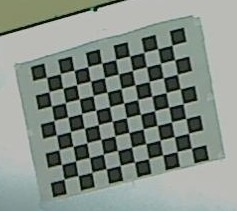
\includegraphics[width=3cm,height=3cm]{../img_source/cam_1.jpg}} &  
\subfloat[]{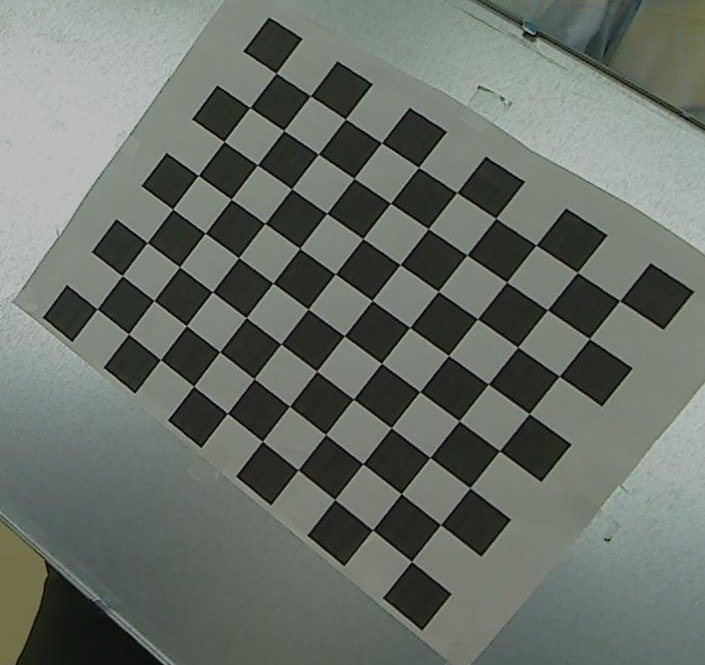
\includegraphics[width=3cm,height=3cm]{../img_source/cam_2.jpg}} &  
\subfloat[]{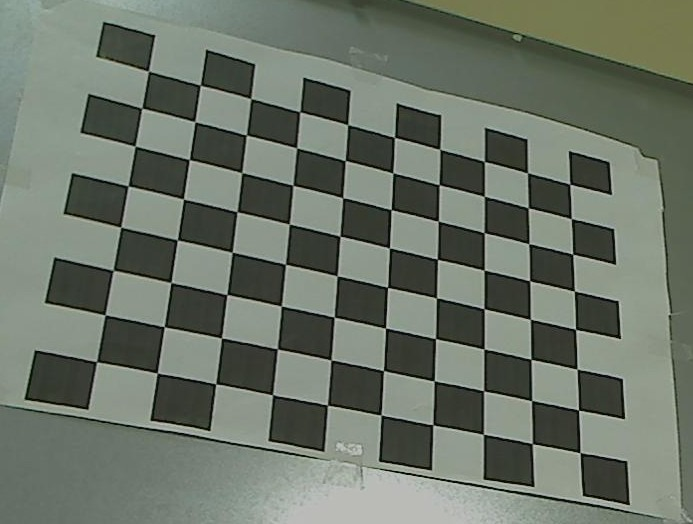
\includegraphics[width=3cm,height=3cm]{../img_source/cam_3.jpg}} &  
\subfloat[]{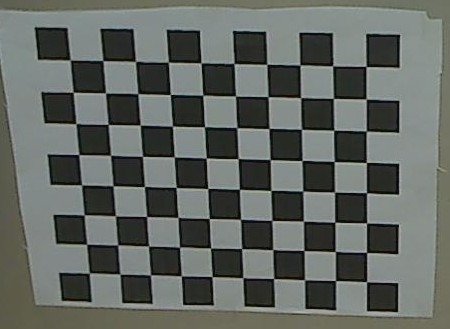
\includegraphics[width=3cm,height=3cm]{../img_source/cam_4.jpg}}\\  
\end{tabular}  
\end{tabularx}  
\caption{Some views used for camera calibration}  
\label{fig:cam_calib_views}
\end{figure}  
Each such view provides a set of 3D-2D correspondence and adds a separate set of rotation and translation parameters to the  
list of unknowns. Since there are 15 unknowns parameters per view hence at least 15 equations needs to be solved for the unknowns. This requires at least 2 views since a single view can provide only 8 constraints(i.e., 4 points are required to completely define a homography). Practically, we use more than 2 views(typically greater than 10) with more than  
4 points per view to account for effect of noise in corner-detection. Acquired 3D-2D point  
correspondences are used to calibrate camera as explained in Section-2.3.  
  
\paragraph{Results and visualization.}  
For visualization of camera calibration process a program to plot the  
views used for calibration was developed. This visualization is similar to [18] but it was not available  
for projector calibration.\newline  
Figures~\ref{fig:cam_calib_plot_1},~\ref{fig:cam_calib_plot_2} show snapshots of 3D plot of all views of checkerboard used for camera  
calibration.  
\noindent  
Here, figure~\ref{fig:cam_calib_plot_1} shows that our calibration range was 50cm to 250cm along Z-axis, -25cm to +45cm along Y-axis.  
\begin{figure}[htbp]  
\centering  
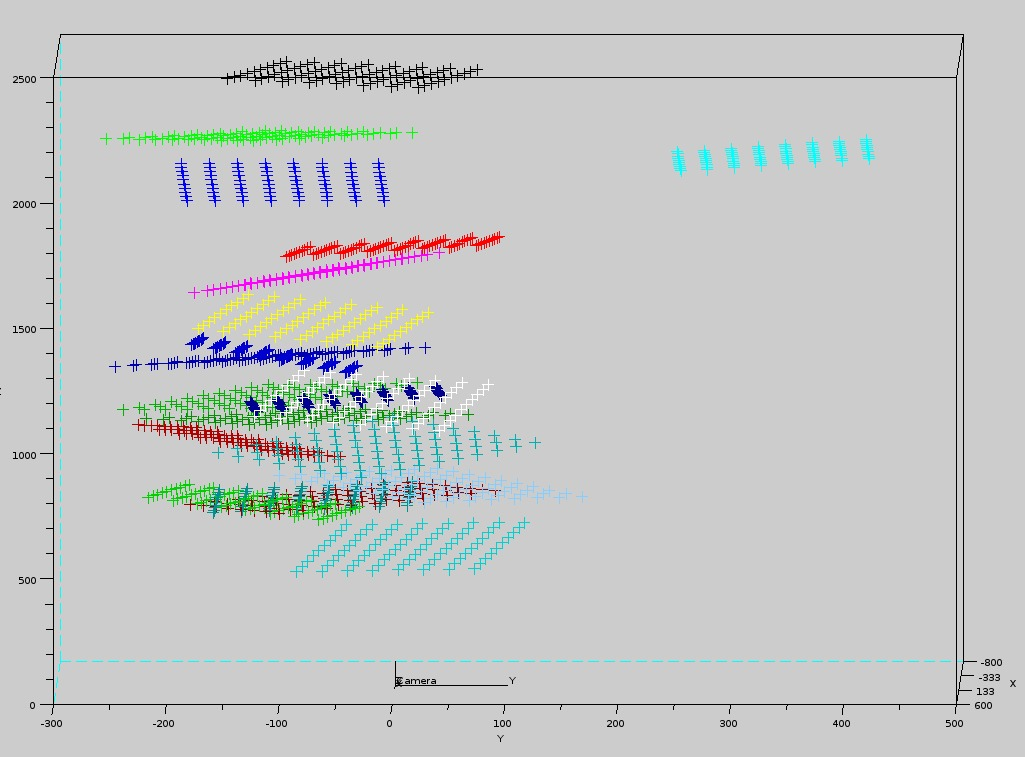
\includegraphics[width=15cm,height=10cm]{../img_source/cam_calib_view.jpg}  
\caption{Visualization of camera calibration results:View along X-axis}  
\label{fig:cam_calib_plot_1}
\end{figure}  
\noindent  
Figure~\ref{fig:cam_calib_plot_2} shows that calibration range along X-axis  
was -50cm just above +40cm. All above mentioned distances are with respect to  
camera coordinates system, which is at (0,0,0) in both figures. So the camera  
calibration volume was approximately 90cm X 70cm X 200cm.  
\begin{figure}[htbp]  
\centering  
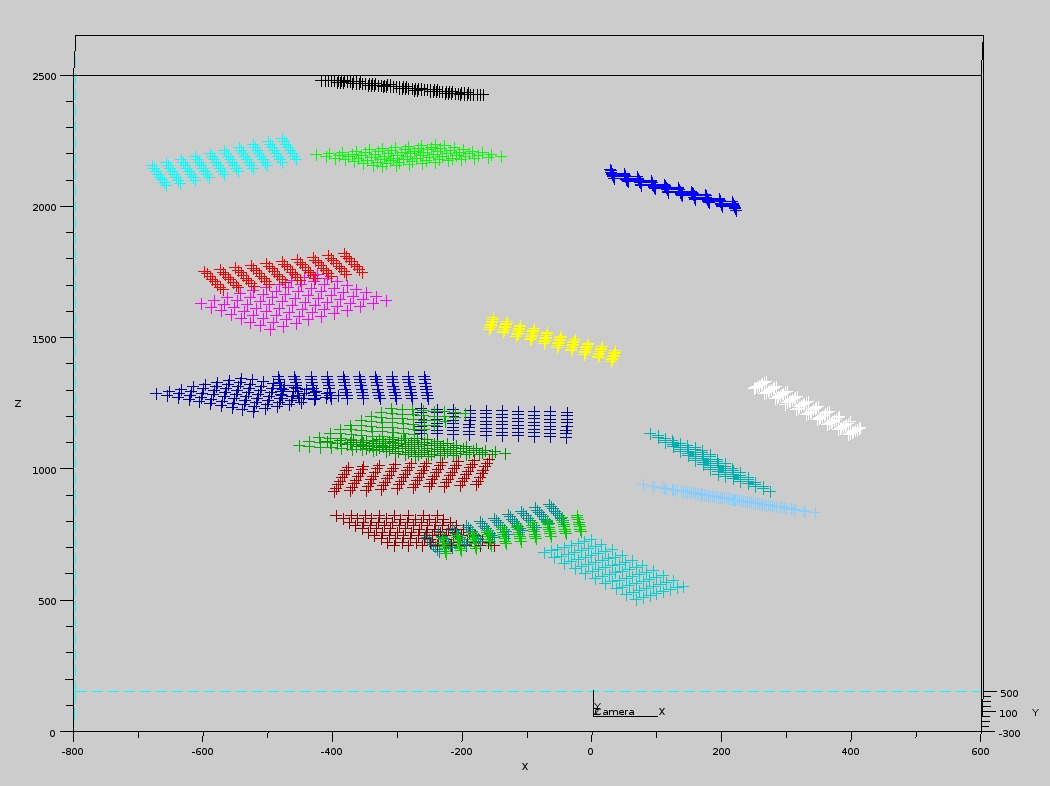
\includegraphics[width=15cm,height=10cm]{../img_source/cam_calib_view2.jpg}  
\caption{Visualization of camera calibration results:View along Y-axis} 
\label{fig:cam_calib_plot_2} 
\end{figure}  
Camera calibration parameters estimated through experiments for Logitech Quickcam sphere AF webcam at native resolution are tabulated in table 2-1. \textit{Reprojection error} mentioned in the table can be defined as a measure of deviation of fitted parameters from the observed world-camera point correspondences.% More formally,  
%\paragraph{Reprojection error.}  
%A measure of accuracy of fitted camera parameters. This is a geometric error, which quantitatively represents the euclidean distance between actual projection of a 3D point(the detected corners) and its projection computed using the estimated parameters.
\begin{table}[hb]  
\centering  
\begin{tabular}{c c}  
\hline\noalign{\smallskip}  
Parameter & Estimated value \\  
\noalign{\smallskip}\hline\noalign{\smallskip}  
$f_x$ & 1362.2\\  
$f_y$ & 1372.2\\  
$c_x$ & 803.9\\  
$c_y$ & 590.1\\  
$k_1$ & 0.07\\  
$k_2$ & -0.14\\  
%$k_3$ & 0.0\\  
%$p_1$ & 0.0\\  
%$p_2$ & 0.0\\  
Reprojection error & 0.20 \\  
\noalign{\smallskip}\hline  
\end{tabular}  
\caption{Estimated Camera intrinsic and distortion model parameters}  
\end{table}   
\subsection{Projector calibration}  
As already mentioned in Section-2.1, projector calibration problem can be regarded as an inverse-camera calibration problem. Consequently, same procedure as of camera calibration has been used to calibrate the projector. Basically, the idea is to use camera as a feedback device which will provide the 3D coordinates for the 2D features projected by the projector, hence providing the 3D-2D point correspondence between world-coordinate system and projector-coordinate system needed for projector calibration similar to camera calibration process.  
  
\paragraph{Procedure:}  
\begin{enumerate}
\item Camera-to-world homography is computed once.
\item For each view,
\begin{enumerate}
\item Projector is physically displaced allowing for rotations and translation with respect to world coordinate system and a checkerboard pattern is projected.  
\item Camera captures the projected features and detects their coordinates. 
\item Using camera-to-world homography, corresponding 3D coordinates are computed.  
\item These 3D coordinates along with the 2D coordinates of projected features(in projector buffer) forms the required 3D-2D correspondence for this view. 
\end{enumerate}
\item After sufficient number of such views(typically greater than 10) are captured projector calibration is performed using same algorithm as for camera calibration.  
\end{enumerate}
  
\noindent   
Figure~\ref{fig:proj_calib_view} shows few views used for projector calibration, projected checkerboard pattern has board dimension 11 squares X 9 squares and has each square of size of 75 pixels X 75 pixels.  
  
\begin{figure}[htbp]  
\centering  
\def\tabularxcolumn#1{m{#1}}  
\begin{tabularx}{\linewidth}{@{}cXX@{}}  
\begin{tabular}{c c c c}  
\hspace{0.8cm}  
\subfloat[]{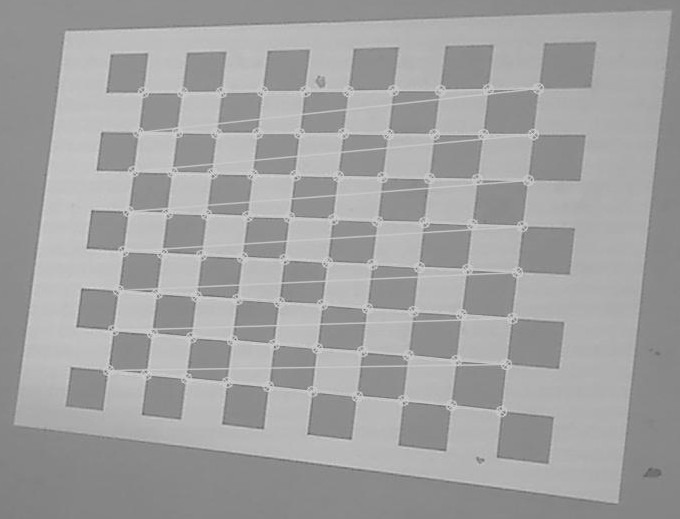
\includegraphics[width=3cm,height=3cm]{../img_source/proj_view_1.jpg}} &  
\subfloat[]{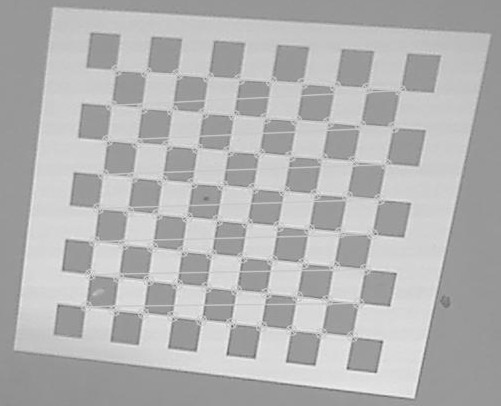
\includegraphics[width=3cm,height=3cm]{../img_source/proj_view_2.jpg}} &  
\subfloat[]{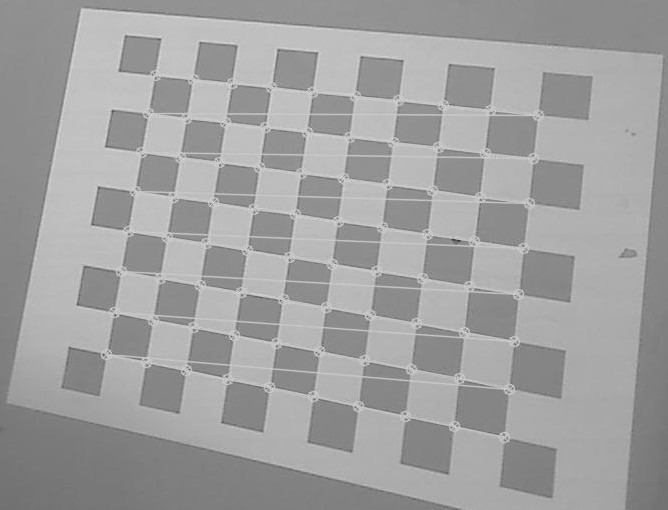
\includegraphics[width=3cm,height=3cm]{../img_source/proj_view_3.jpg}} &  
\subfloat[]{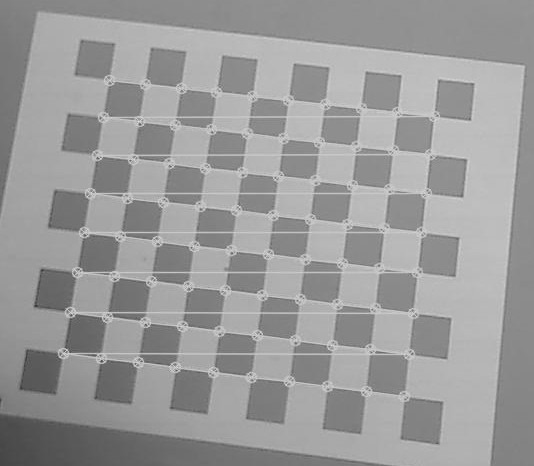
\includegraphics[width=3cm,height=3cm]{../img_source/proj_view_4.jpg}} \\  
\end{tabular}  
\end{tabularx}  
\caption{Some view used for projector calibration} 
\label{fig:proj_calib_view} 
\end{figure}  
  
  
\paragraph{Results and visualization.}  
Calibration parameters for Sharp PG F200X projector computed by performing above mentioned procedure are tabulated in table 2.2.  
\begin{table}[htbp]  
\centering  
\begin{tabular}{c c}  
\hline\noalign{\smallskip}  
Parameter & Estimated value \\  
\noalign{\smallskip}\hline\noalign{\smallskip}  
$f_x$ & 2261.7\\  
$f_y$ & 2262.8\\  
$c_x$ & 522.7\\  
$c_y$ & 713.8\\  
%$k_1$ & 0.0\\  
%$k_2$ & 0.0\\  
%$k_3$ & 0.0\\  
%$p_1$ & 0.0\\  
%$p_2$ & 0.0\\  
\noalign{\smallskip}\hline  
\end{tabular}  
\caption{Estimated Projector intrinsic model parameters}  
\end{table}  
\noindent  
Figures~\ref{fig:proj_calib_plot_1}, ~\ref{fig:proj_calib_plot_2} show plots of views used for projector calibration.Here, figure~\ref{fig:proj_calib_plot_1} shows that calibration range for along X-axis is -100cm to +150cm along Z-axis it is -50cm to +250cm.  
\begin{figure}[htbp]  
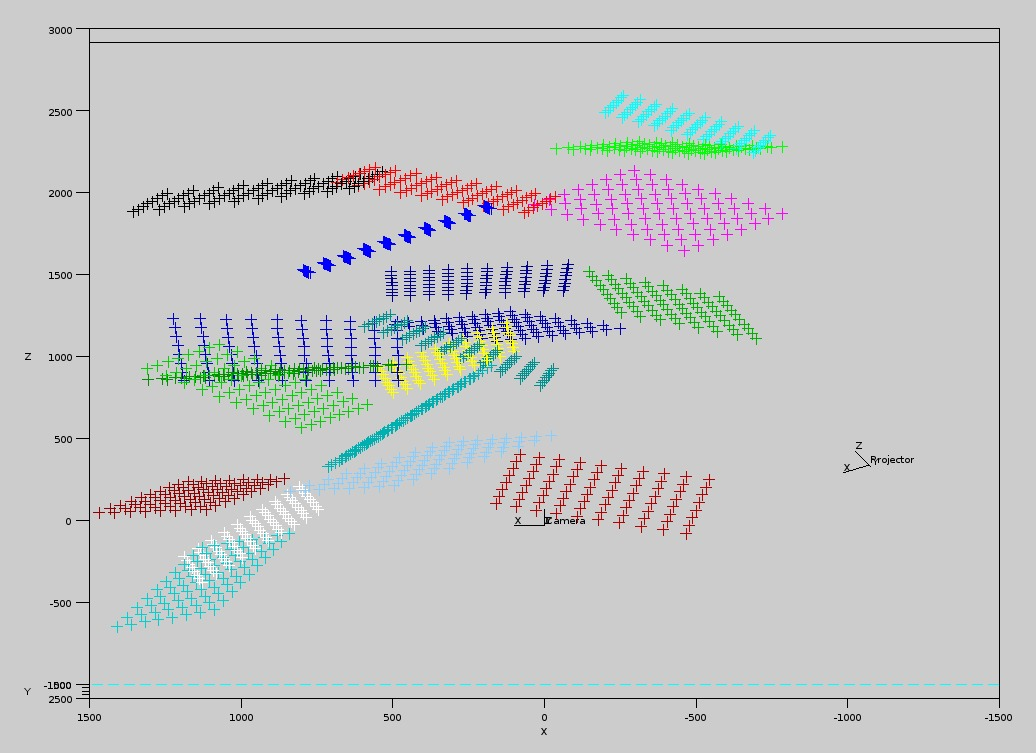
\includegraphics[width=15cm,height=10cm]{../img_source/proj_calib_plot_1.jpg}   
\caption{Visualization of projector calibration views along Y-axis} 
\label{fig:proj_calib_plot_1} 
\end{figure}  
\noindent  
Figure~\ref{fig:proj_calib_plot_2} shows calibration range along Y-axis to be from -125cm to +225cm.All measurements are with respect to camera-coordinate system which is shown at (0,0,0) in the figures. Hence calibration volume for projector was 250cm X 400cm X 300cm.  
\begin{figure}[htbp]  
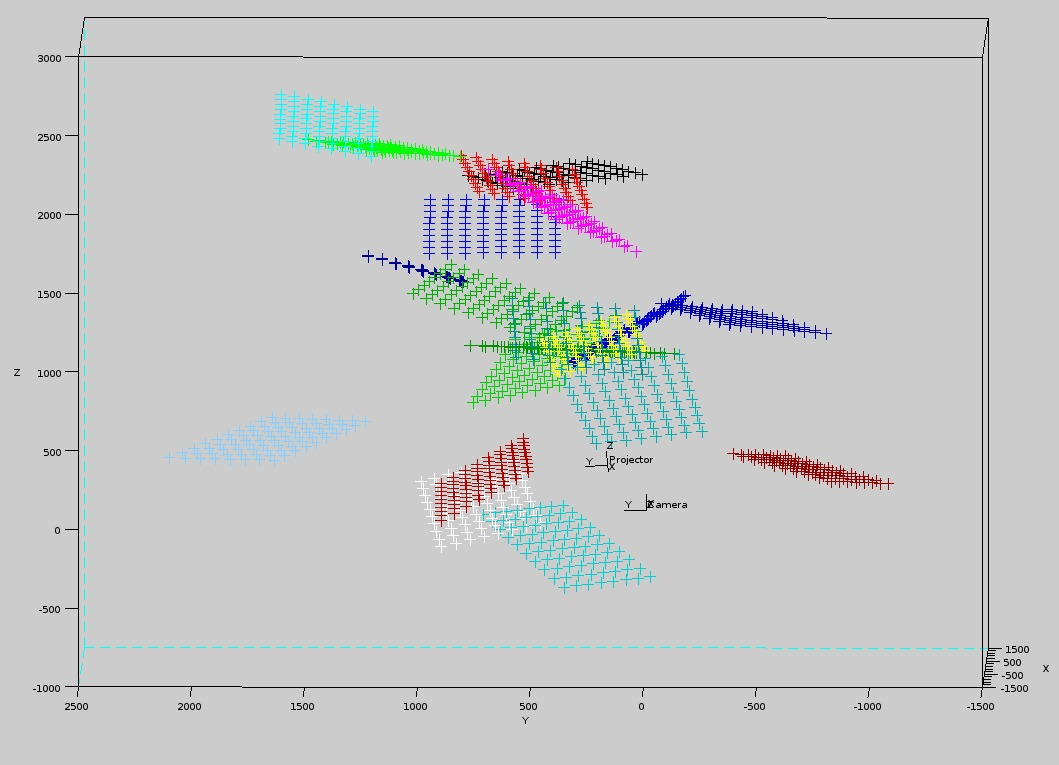
\includegraphics[width=15cm,height=10cm]{../img_source/proj_calib_plot_2.jpg}  
\caption{Visualization of projector calibration views along X-axis}  
\label{fig:proj_calib_plot_2}
\end{figure}  
  
  
  
  
  
\subsection{Camera-projector relative extrinsic calibration}   
As mentioned in an end note in section 2.3, relative calibration of projector with respect to camera is needed to bring both projector and camera to a common coordinate system which is a implicit assumption in triangulation. In this work, extrinsic calibration function available in OpenCV to determine the extrinsic parameters(i.e., rotation translation of projector coordinate system with respect to camera coordinate system) was used.  Rigid body transformations of camera and projector coordinate systems with respect to world coordinate system allow for determining the transformations between them(refer Note on relative calibration in section-2.3 for underlying equations)  
  
  
\paragraph{Procedure:}
\begin{enumerate} 
\item Extrinsic calibration of camera with respect to world coordinate system:  
\begin{enumerate}
\item A known reference plane(whose dimensions are known) containing world coordinate system is captured and corners are detected.  
\item These detected features are used for computing camera-to-world homography.  
\item Using the 3D-2D correspondences determined above, extrinsic calibration of camera is performed.  
\end{enumerate}
\item Extrinsic calibration of projector with respect to world coordinate system:  
\begin{enumerate}
\item Projector projects a checkerboard pattern, which is captured by the camera.  
\item Using the camera-to-world homography computed above, 3D coordinates for the projected feature points can be computed.  
\item These  3D-2D correspondences(3D coordinates of projected feature points and corresponding 2D coordinates in projector image) are used for computing relative rotation and translation of projector coordinate system with respect to world coordinate system.  
\end{enumerate}
\item Relative rotation and translation of projector coordinate system with respect to camera coordinate system is computed(refer Note on relative calibration in section 2.3 for underlying equations)  
\end{enumerate}  
  
\paragraph{Results and visualization.}  
Estimated extrinsic calibration parameters for a sample camera-projector geometry are tabulated in table 2.3,2.4,2.5.It should be noted however that these results are for one specific system configuration and do not represent any intrinsic characteristic of system. Hence they are called extrinsic parameters.\newline  

 
In tables~\ref{table:cam_extrinsics}.~\ref{table:proj_extrinsics},~\ref{table:cam_proj_extrinsics},  
$(r_1^{wc},r_2^{wc},r_3^{wc})$ is rotation transformation from world coordinate system to camera coordinate system  
$(t_1^{wc},t_2^{wc},t_3^{wc})$ is translation transformation from world coordinate system to camera coordinate system  
$(r_1^{wp},r_2^{wp},r_3^{wp})$ is rotation transformation from world coordinate system to projector coordinate system  
$(t_1^{wp},t_2^{wp},t_3^{wp})$ is translation transformation from world coordinate system to projector coordinate system  
$(r_1^{pc},r_2^{pc},r_3^{pc})$ is rotation transformation from projector coordinate system to camera coordinate system  
$(t_1^{pc},t_2^{pc},t_3^{pc})$ is translation transformation from projector coordinate system to camera coordinates system. Rotation vectors are expressed in radians in axis-angle form, translation is expressed in `mm'.\newline  
\begin{table}[ht]  
\parbox{.45\linewidth}{  
\centering  
\begin{tabular}{c c}  
\hline\noalign{\smallskip}  
Parameter & Estimated value \\  
\hline  
$r_1^{wc}$ & 0.128 \\  
$r_2^{wc}$ & 0.239 \\  
$r_3^{wc}$ & 0.035\\  
$t_x^{wc}$ & -920.7\\  
$t_y^{wc}$ & -834.6\\  
$t_z^{wc}$ & 2960.6\\  
\hline  
\end{tabular}   
\caption{Estimated camera extrinsic parameters}
\label{table:cam_extrinsics}
}  
\hfill  
\parbox{.45\linewidth}{  
\centering  
\begin{tabular}{c c}  
\hline\noalign{\smallskip}  
Parameter & Estimated value \\  
\hline  
$r_1^{wp}$ & -0.047 \\  
$r_2^{wp}$ & -0.246 \\  
$r_3^{wp}$ & 0.008\\  
$t_x^{wp}$ & -1054.0\\  
$t_y^{wp}$ & -1235.0\\  
$t_z^{wp}$ & 2281.0\\  
\hline  
\end{tabular}  
\caption{Estimated projector extrinsic parameters}  
\label{table:proj_extrinsics}
}\\  

\parbox{.45\linewidth}{
\centering  
\begin{tabular}{c c}  
\hline\noalign{\smallskip}  
Parameter & Estimated value \\  
\hline  
$r_1^{pc}$ & -0.086 \\  
$r_2^{pc}$ & 0.484 \\  
$r_3^{pc}$ & 0.006\\  
$t_x^{pc}$ & -1080.3\\  
$t_y^{pc}$ & 188.9\\  
$t_z^{pc}$ & 359.4\\  
\hline  
\end{tabular}  
\caption{Estimated projector-camera relative parameters}  
\label{table:cam_proj_extrinsics}
}  
\end{table}  
  
\noindent  
View used for extrinsic calibration of projector camera system is depicted in Figure~\ref{fig:extrinsic_calib_setup}. Figure~\ref{fig:extrinsic_plot} shows the plan-view of estimated projector-camera-world configuration.In figure~\ref{fig:extrinsic_plot} `green' object is the top-view of projected checkerboard. Estimated positions of world-coordinate system, projector-coordinate system and camera-coordinate system are also shown.   
\begin{figure}[htbp]  
\centering  
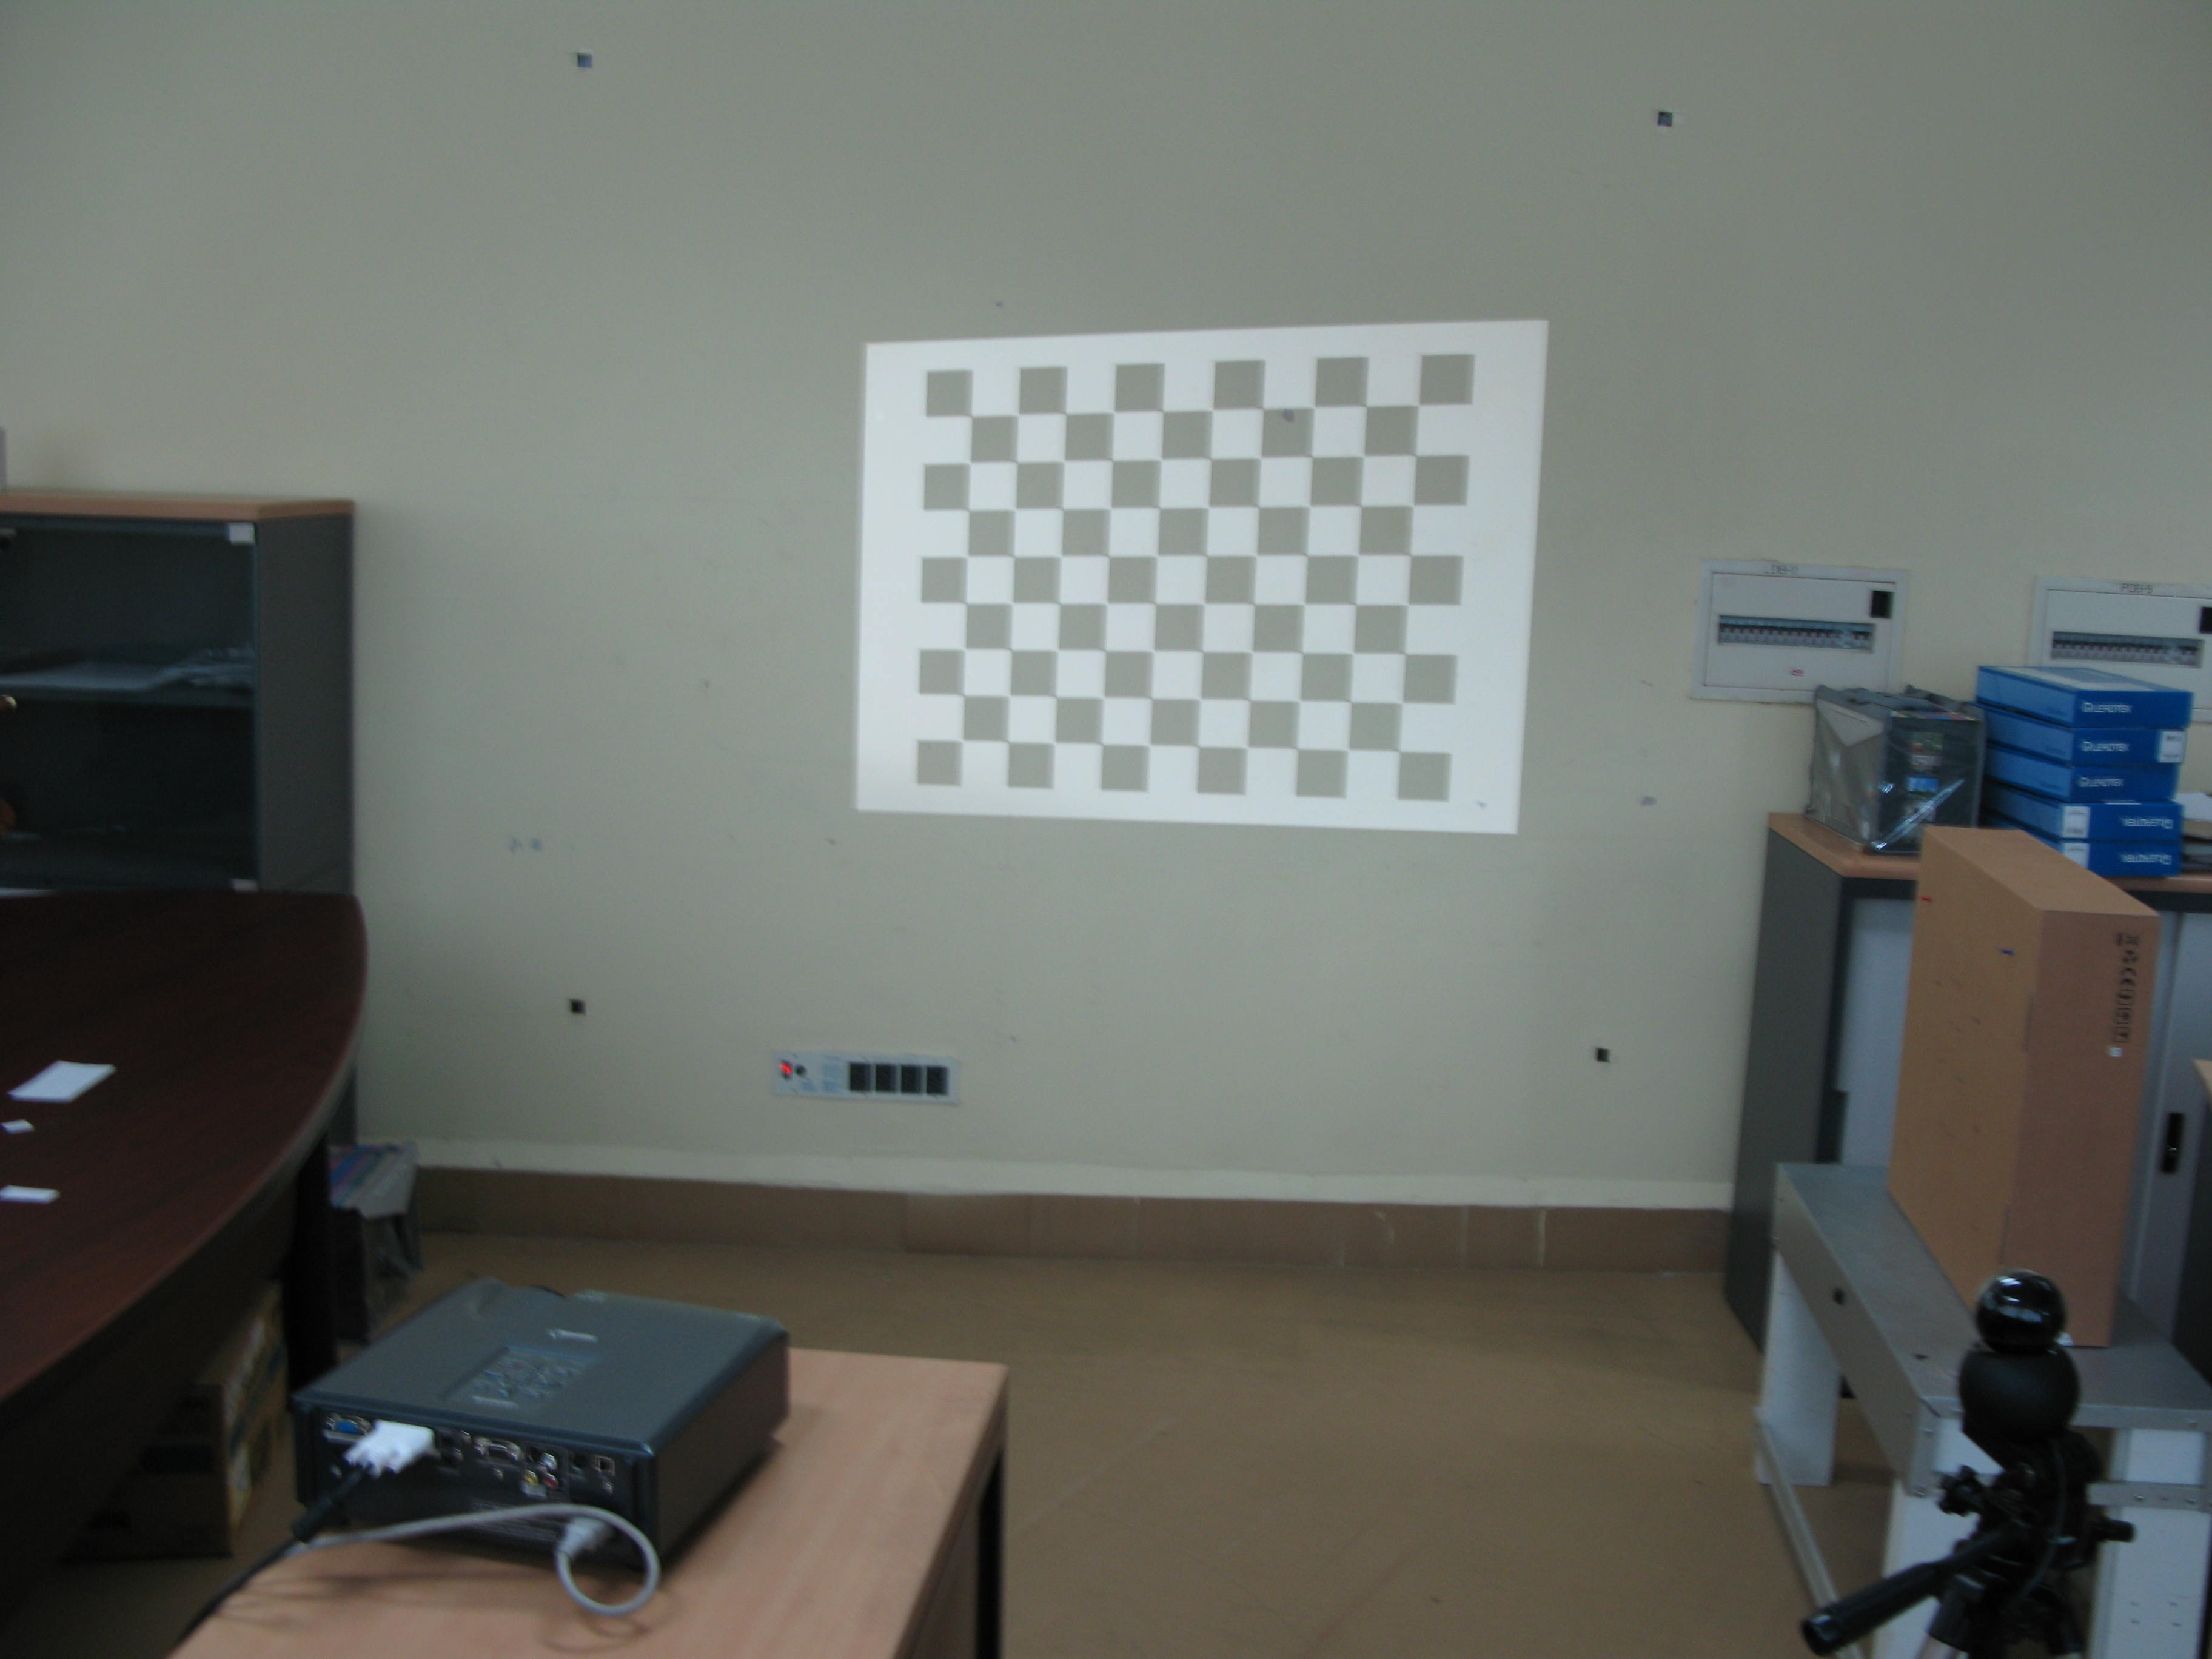
\includegraphics[width=7cm,height=5.5cm]{../img_source/system_extrinsic.jpg}  
\caption{Actual setup for extrinsic calibration}  
\label{fig:extrinsic_calib_setup}
\end{figure}  
  
\begin{figure}[!htbp]  
\centering  
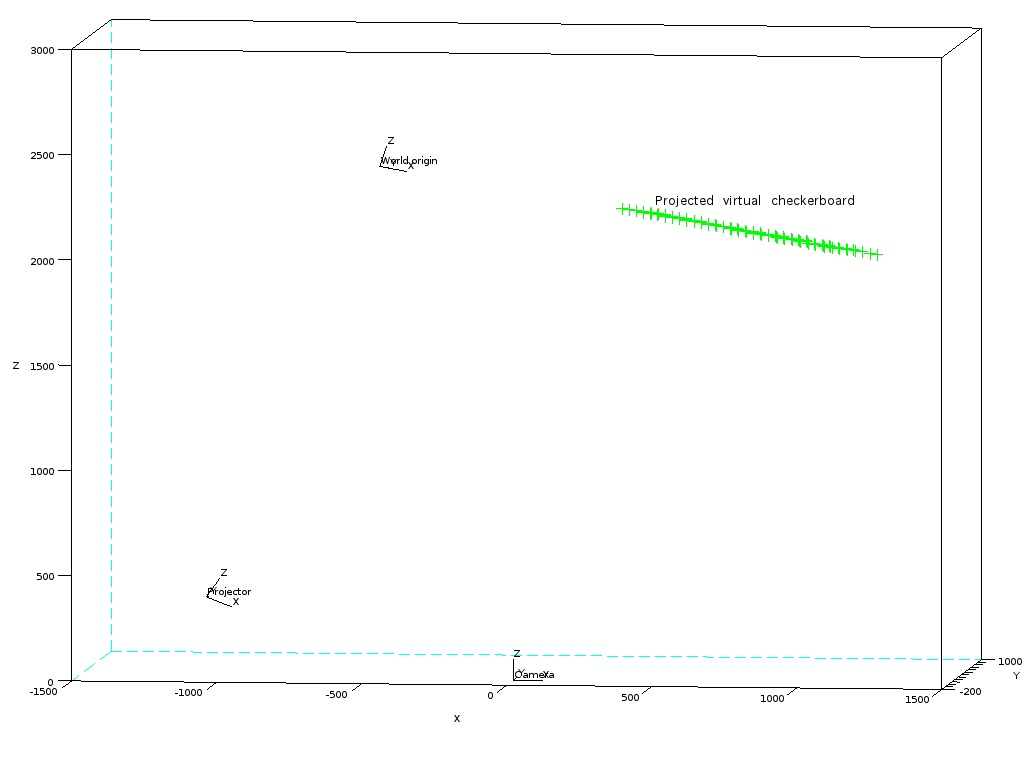
\includegraphics[width=17cm,height=11.3cm]{../img_source/system_plot_edit.jpg}  
\caption{Estimated system extrinsic geometry}  
\label{fig:extrinsic_plot}
\end{figure}  
\noindent  
 
  
\section{Discussion}  
During camera calibration it was observed that for larger distances($\sim2m$) of calibration board from camera, sub-pixel corner detection algorithm gives inaccurate results. Further, there has been no study on optimal \textit{window size} and \textit{termination criteria} for sub-pixel corner detection algorithm in the literature due to which these parameters were decided experimentally.\newline  
\indent Projector calibration using OpenCV camera calibration algorithm gives non-repeat-able estimated parameters of which reason is still unknown and deserves further study.\newline  
\indent It was observed that there are certain camera-projector geometric configurations for example when base-line between optical centers of camera and projector is small, for which OpenCV pose-estimation gives degenerate results, again this problem needs further study.   
  
  
\section{Summary}  
In this chapter, camera model was described as a series of transformations on a real world 3D point. In review, currently most popularly used calibration algorithms were briefly described. Further, working of the developed system calibration module was described with individual explanations of used procedure for camera, projector and relative extrinsic calibration. To make calibration results more comprehensive, individual plots for camera, projector and relative extrinsic calibration process were presented.
 

